\label{chapter: phase sep}

From now one and for simplicity, we will restrict the presentation to the case of a scalar mobility $M(\phi) > 0$.

\noindent {\it Spinodal decomposition} First, we can investigate the condition for a homogeneous configuration with $\phi = \bphi$ to be linearly stable.
Writing $\phi(\bm r,t) = \bphi + \delta \phi(\bm r,t)$, the perturbations $\delta \phi(\bm r,t)$ obey at linear order
\begin{equation} \label{eq_linear_phi}
\partial_t \delta \phi(\bm r,t) = \bar{M} \nabla^2 \left[ \left( \bar{f}'' - \bar{\kappa} \nabla^2\right)\delta \phi(\bm r,t)\right],
\end{equation}
where the bars stand for quantities evaluated at $\bphi$. 
Going into Fourier space, the growth rate associated to the mode with wavenumber $q$ is therefore $\lambda_q = -\bar{M} q^2(\bar{f}'' + \bar{\kappa} q^2)$.
As $\bar{M}$ and $\bar{\kappa}$ are both positive, the homogeneous configuration becomes unstable whenever $\bar{f}'' < 0$. 
This condition defines the so-called spinodals in the $(\bphi, k_B T$) phase diagram (Fig.~\ref{figeq}). 

%%%%%%%%%%%%%%%%%%%%%%%%%%%%
\begin{figure}[ht!]
	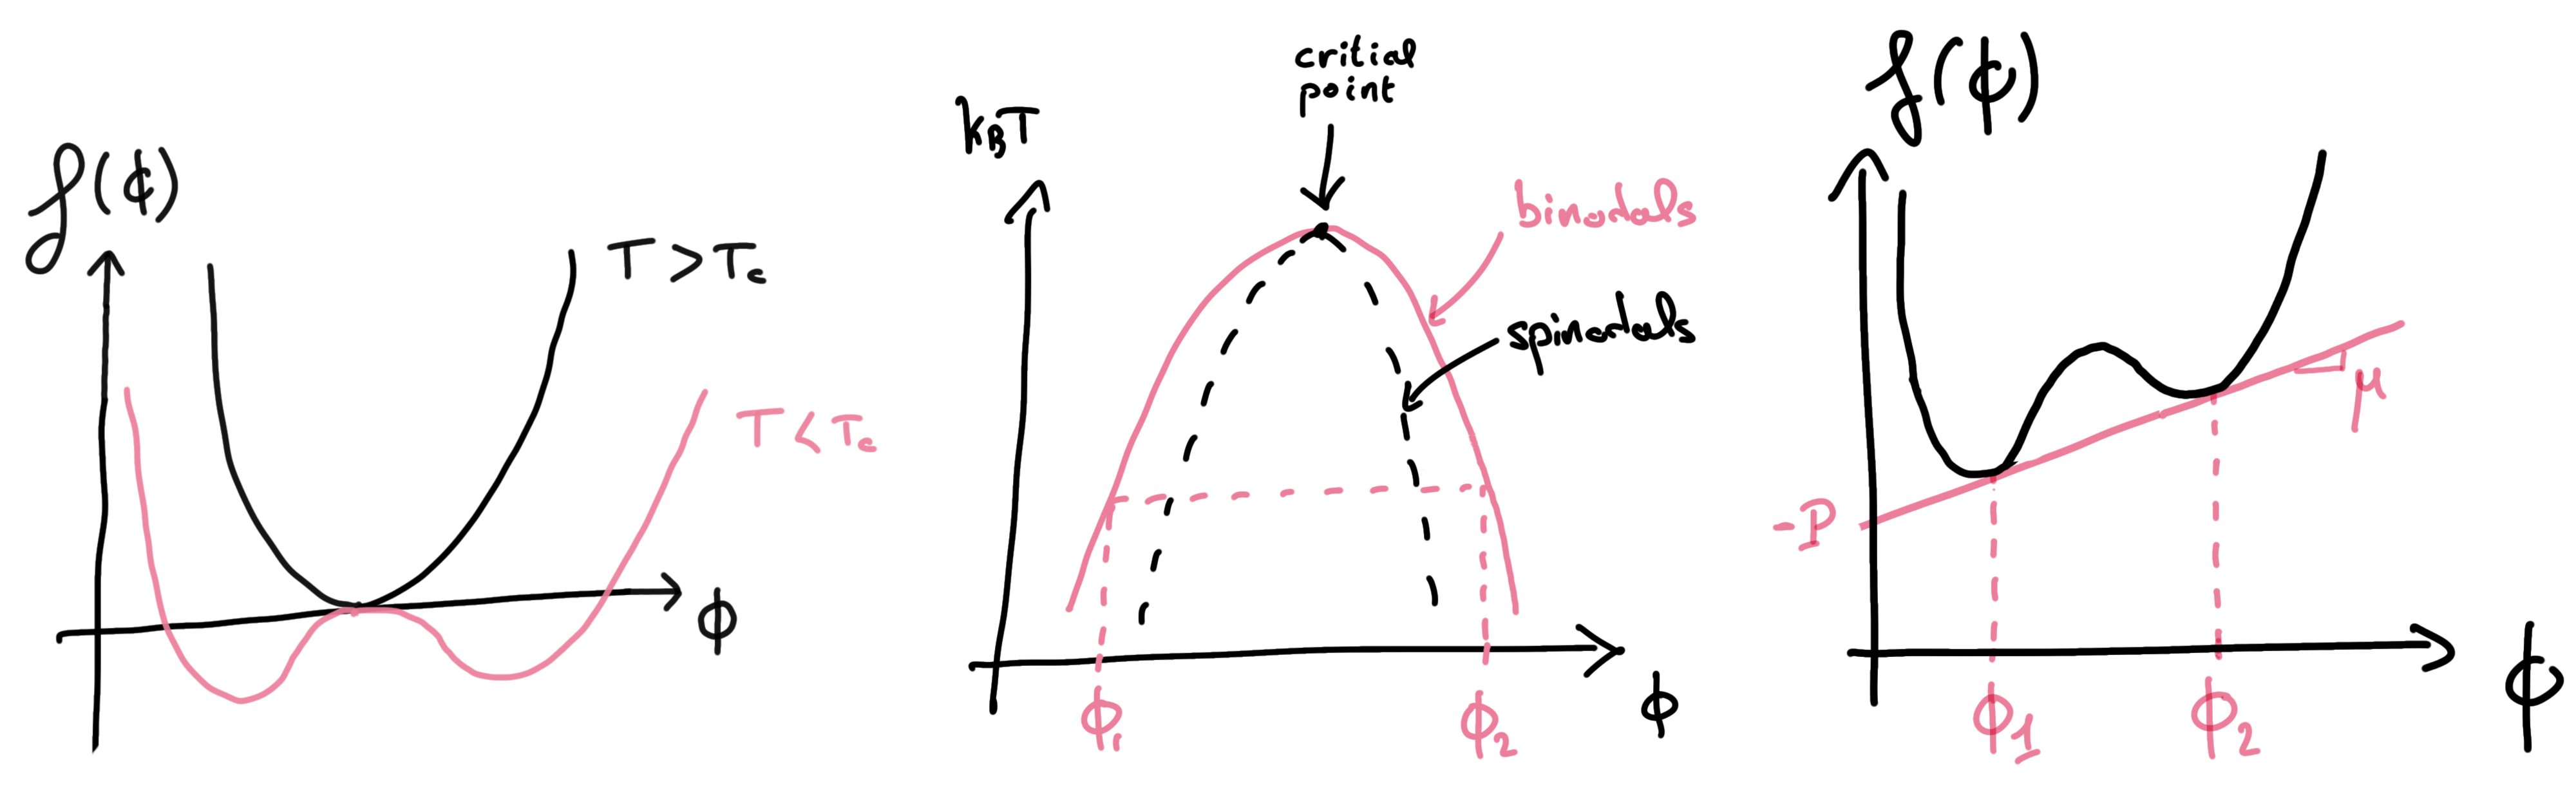
\includegraphics[width=\textwidth]{Figures/equilibrium_ps.pdf}
	\caption{Left: Typical Landau free energy landscapes above and below the critical point. 
	Center: phase diagram in the temperature $\phi$ plane showing the spinodals, binodals and critical point. 
	Right: Common tangent construction allowing to determine the coexistence densities in the phase separated regime.}
	\label{figeq}
\end{figure}
%%%%%%%%%%%%%%%%%%%%%%%%%%%%

\noindent {\it Binodals and the composition of phase separated configurations} 
The linear stability analysis and determination of the spinodals does not tell us anything about the asymptotic ($t \to \infty$) state of the system.
After the system undergoes spinodal decomposition, it goes through a coarsening regime until it phase separates into coexisting domains with different volumes and densities.
To determine the coexisting densities, we use the conservations of the total volume ${\cal V}$ and of the field $\phi$. 
We moreover work in the thermodynamic limit ${\cal V} \to \infty$ such that contributions from the interfaces can be safely neglected and we only consider the bulk contribution $f(\phi)$.
In a stationary phase separated regime where the system is partitioned into two domains with $\phi = \phi_{1,2}$ and of respective volumes ${\cal V}_{1,2}$, 
the free energy~\eqref{eq_F} thus takes the form
\begin{equation} \label{eq_F_ps}
{\cal F} = f(\phi_1) {\cal V}_1 + f(\phi_2) {\cal V}_2,
\end{equation} 
while denoting the mean value of $\phi$ as $\bphi$ the conservation constraints give
\begin{equation} \label{eq_constraints_binodals}
\phi_1 {\cal V}_1 + \phi_2 {\cal V}_2 = \bphi {\cal V}, \qquad  {\cal V}_1 + {\cal V}_2 = {\cal V} .
\end{equation} 
To determine the values $\phi_1$ and $\phi_2$, we can thus minimize the free energy~\eqref{eq_F_ps} imposing~\eqref{eq_constraints_binodals}.
This is done by adding the Lagrange multipliers ($\mu,P$) to ${\cal F}$, such that we define $\tilde{\cal F} = {\cal F} + P({\cal V}_1 + {\cal V}_2) - \mu(\phi_1 {\cal V}_1 + \phi_2 {\cal V}_2)$.
Minimizing $\tilde{\cal F}$ wrt the values of $\phi$ and volume for each of the two populations, we get
\begin{align} \label{eq_binodal_mu}
\frac{\partial \tilde{\cal F}}{\partial \phi_i}  & = {\cal V}_i (f'(\phi_i) - \mu) = 0 , \\
\label{eq_binodal_P}
\frac{\partial \tilde{\cal F}}{\partial {\cal V}_i}  & = f(\phi_i) - \mu \phi_i + P = 0 ,
\end{align}
with $i = 1,2$.
Eq.~\eqref{eq_binodal_mu} thus imposes that the chemical potential $\mu = f'(\phi_1) = f'(\phi_2)$ takes identical values in both phases (\emph{diffusive equilibrium}),
while Eq.~\eqref{eq_binodal_P} ensures the equality of pressures (\emph{mechanical equilibrium}).
Therefore, one can thus determine graphically the values of $\phi_1$ and $\phi_2$ from a common tangent construction 
on the free energy landscape. 
Indeed, the equality of chemical potentials imposes equal slopes of $f$ at $\phi_1$ and $\phi_2$, 
while equality of pressures imposes a common intercept on the vertical axis as shown in Fig.~\ref{figeq}

Varying e.g.\ the system temperatures, the coexistence values $\phi_{1,2}$ define the \emph{binodal curves},
and meet the spinodals we determined previously at the critical point. 
As shown in Fig.~\ref{figeq}, the spinodals and binodals generally do not coincide, such that there are regions of the phase diagram 
where phase separated configurations exist (and are stable) but the homogeneous state at $\phi = \bphi$ is also linearly stable.
In practice, if we now put back noise into the picture in these regions the homogeneous state will typically disappear 
not through the deterministic growth of an infinitesimal perturbation, 
but because of stochastic nucleation events which correspond to large perturbations and thus cannot be captured by linear stability analysis.
At fixed temperature below $T_c$ and for $\bphi$ lying in between the binodals, the system thus always phase separates over long times into two distinct domains 
where $\phi$ takes values $\phi_{1,2}$ and whose volumes linearly interpolate between 0 and ${\cal V}$ for $\bphi \in [\phi_1;\phi_2]$ due to the condition~\eqref{eq_constraints_binodals}, 
namely
\begin{equation}
{\cal V}_1 = \frac{\phi_2 - \bphi}{\phi_2 - \phi_1} {\cal V}, \qquad {\cal V}_2 = {\cal V} - {\cal V}_1 = \frac{\bphi - \phi_1}{\phi_2 - \phi_1} {\cal V},
\end{equation} 
which is known as the \emph{lever rule}.\\

\noindent {\it The coarsening dynamics} So far, we have discussed the linear instability of homogeneous solutions and the relative composition of phase separated phases.
Of course, another interesting aspect of phase separation concerns how one moves from one to the other. 
Without entering into details (for the interested reader see~\cite{Bray1994}), 
the coarsening process leading to phase separation can be understood by taking into account finite size effects, 
i.e.\ by considering the nonlocal contributions to the free energy which were neglected above.
Doing this, one finds that the pressure inside a spherical droplet increases with its interface curvature, 
leading to a diffusive flux from small to large droplets. 
Over long times, small droplets thus typically shrink at the expense of larger ones which is known as \emph{Ostwald ripening}.
One can moreover show that under this process the mean droplet radius universally grows as $\sim t^{1/3}$,
while the asymptotic ($t \to \infty$) state inevitably consists of two macroscopic phase separated domains. 














\section{Passive model B and Cahn-Hilliard dynamics}

\label{sec_PMB}

\subsection{The dynamical theory for conserved scalar order parameter} 

We learned from statistical mechanics that the large-scale dynamics of systems that microscopically obey detailed balance minimize a free energy.
Therefore, model B is generally written in terms of a functional ${\cal F}[\phi]$, whose expression can be generally\footnote{You can consider other terms up to order $|\nabla \phi|^2$, 
and then think of why they cannot be allowed in the expression of ${\cal F}$.} expressed as
%
\begin{equation} \label{eq_F}
{\cal F}[\phi] = \intd{r} \left[ f(\phi) + \frac{\kappa(\phi)}{2}|\nabla\phi|^2\right],
\end{equation} 
%
where we have kept terms up to order $|\nabla \phi|^2$.
In Eq.~\eqref{eq_F} $f$ denotes the `bulk' free energy density and $\kappa(\phi) > 0$ a generic constant.
The bulk contribution consists of a free energy landscape due to e.g.\ entropic effects and interactions between microscopic elements, 
while the $\kappa$ term describes the cost of interfaces.

The dynamical equation for $\phi$ then takes the general form
\begin{equation} \label{eq_phi}
\partial_t \phi(\bm r,t) = - \nabla \cdot \bm J(\phi) ,
\end{equation}
where the current $\bm J = \bm J_{\rm D} + \bm J_{\rm S}$ has a deterministic and stochastic contributions.
$\bm J_{\rm D}$ is set by the chemical potential:
\begin{equation} \label{eq_JD}
\bm J_{\rm D}(\phi) = - \bm M(\phi) \cdot \nabla \mu(\phi), \qquad \mu(\phi) = \frac{\delta {\cal F}}{\delta \phi} = f'(\phi) - \kappa(\phi) \nabla^2\phi - \frac{\kappa'(\phi)}{2}|\nabla\phi|^2 .
\end{equation}
The stochastic part $\bm J_{\rm S}$ can be determined using the fluctuation dissipation relation:
\begin{equation} \label{eq_JS}
\bm J_{\rm S}(\bm r,t) = \sqrt{2 k_B T} \bm \sigma(\phi) \cdot \bm \Lambda(\bm r,t), \qquad \Lambda_i(\bm r,t)\Lambda_j(\bm r',t') = \delta_{ij}\delta^d(\bm r - \bm r')\delta(t - t'),
\end{equation}
with $\sigma_{ik}(\phi)\sigma_{jk}(\phi) = M_{ij}(\phi)$ (Einstein summation is implied).

\noindent {\it Exercise: Show that Eqs.~(\ref{eq_phi}-\ref{eq_JS}) imply the stationary Boltzmann distribution ${\cal P}_{\rm s}[\phi] = \exp\left(-\tfrac{{\cal F}[\phi]}{k_B T} \right)$ for the stochastic field $\phi$. 
Hint: the Fokker-Planck equation associated with~\eqref{eq_phi} is given by 
\begin{equation*}
\partial_t {\cal P}[\phi,t] = \intd{x} \frac{\delta}{\delta \phi}\left[ \nabla \cdot \left( {\cal P}[\phi,t] \bm J_{\rm D} - k_B T \bm M(\phi) \cdot \nabla \frac{\delta}{\delta \phi} {\cal P}[\phi,t]  \right) \right] .
\end{equation*}
}

The stochastic contribution to Eq.~\eqref{eq_phi} is usually written to study dynamical effects due to fluctuations (such as the roughening of interfaces, or when one studies critical points using the dynamical renormalization group). In these lectures we will focus on the mean field properties of the models and thus drop the contribution from the noise ($\bm J_{\rm S} = \bm 0$).

In these notes, we will keep the expression of the free energy density $f(\phi)$ general. 
Its expression of course depends on the model of interest, below we describe two popular ones: 
\begin{itemize}
\item {\bf The Flory-Huggins theory of polymer solutions.} Considering polymers in a solvent with respective volume fractions $\phi = v \rho$ and $\phi_{\rm sol} = v_{\rm sol} \rho_{\rm sol}$, 
the incompressibility of the solution implies that $\phi + \phi_{\rm sol} = 1$.
The Flory-Huggins free energy is then given by
$f_{\rm FH}(\phi) = k_B T \left[ \tfrac{1}{v} \phi \ln(\phi) + \tfrac{1}{v_{\rm sol}} (1-\phi)\ln(1-\phi) \right] + \chi \phi(1-\phi)$ where the first term accounts for the entropy contribution due to mixing of the polymer in the solvent, while the second term ($\propto \chi$) accounts for interactions. In the case where the latter are attractive, $\chi < 0$. For more details see e.g.~\cite{Eisele1990}. 
\item {\bf Cahn-Hilliard (Landau).} In general, the free energy can expanded in powers of $\phi$: $f_{\rm CH}(\phi) = \sum_i \tfrac{a_k}{k}\phi^k$ with the $\{a_k\}$ real coefficients allowed by the symmetries of the problem. 
Such expansion is generally considered as formally valid close to a critical point where $\phi$ is small (typically $\phi = (\rho - \rho_c)/\rho_c$) such that one usually truncates it at order $k = 4$.
Note that $f_{\rm CH}$ can be obtained from $f_{\rm FH}$ by expanding the logarithms.
\end{itemize}







